\chapter{Results}

\section{Data sets}
In the following we will use two different datasets

\begin{figure}
    \centering
    \begin{subfigure}[b]{0.45\textwidth}
        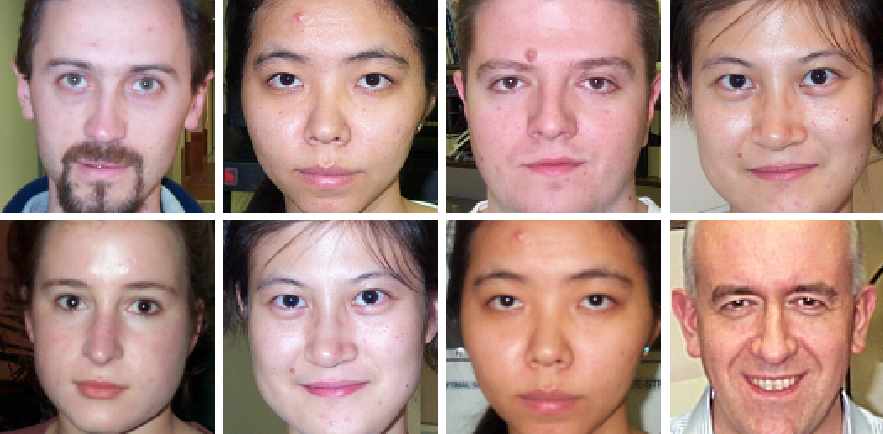
\includegraphics[width=\textwidth]{fig/data/caltech}
        \caption{ Caltech dataset}
    \end{subfigure}
    ~
    \begin{subfigure}[b]{0.45\textwidth}
        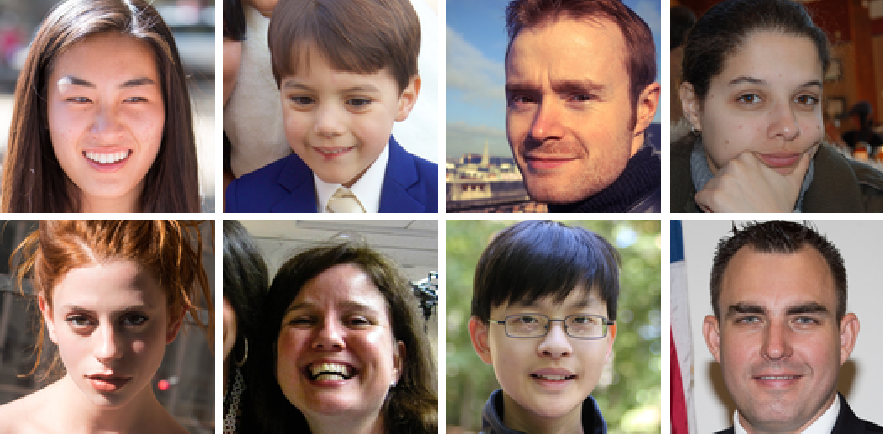
\includegraphics[width=\textwidth]{fig/data/ffhq}
        \caption{FFHQ dataset}
    \end{subfigure}

    \caption{The raw data from the Caltech and FFHQ datasets respectively. This figure is the only one containing images of real people in the report.}
    \label{rawdata}
\end{figure}


\section{Principal Component Analysis }
In this section we explore the results of using Principal Component Analysis (PCA) for face synthesis. PCA is predominately used for dimensionality reduction but here we will use it for synthesis.

The goal of PCA is to find the Principal Components which are the directions of greatest variance in the dataset. These directions are the eigenvectors or, in this context, eigenfaces of the covariance matrix.

Let $\tilde{\mathbf{X}} = \mathbf{X} - \bar{\mathbf{X}}$ then $\mathbf{X}^T\mathbf{X}$ is the covariance matrix we find the eigenfaces the usual way by demanding that $\det(\mathbf{X}^T\mathbf{X} - \lambda) = 0$
We then sort the eigenface after eigenvalue $\lambda$ in order of descending variance. In Figure \ref{eigenface} we see the first 8 eigenfaces.

\begin{figure}
  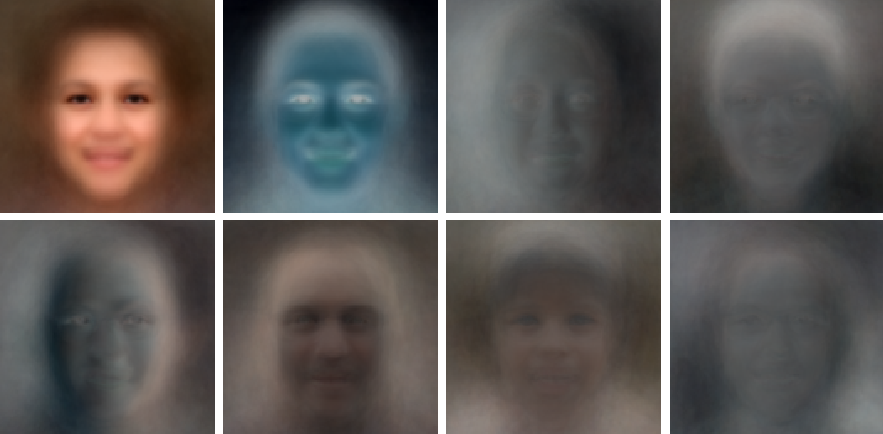
\includegraphics[width=\textwidth]{fig/PCA/pca}
  \caption{Eigenfaces of the FFHQ dataset.}
  \label{eigenface}
\end{figure}

We can generate new synthetic faces $F$ by adding a linear combination of the
eigenfaces $F_i$ to the mean face $F_m$.

\begin{align}
F  = F_m + \sum_{i} \alpha_i F_i
\end{align}
in Figure \ref{pca-components} we see the results of varying the first six
principal components.

In order it seems that the Principal Component control aspects of 1) and 2) Color 3) direction of lighting 4) age 5) pose and 6) gender.


\begin{figure}
    \centering
    \begin{subfigure}[b]{\textwidth}
        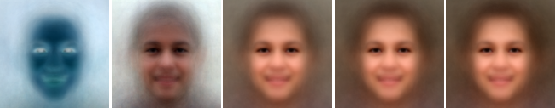
\includegraphics[width=\textwidth]{fig/PCA/pca0}
        \caption{First Principal Component}
    \end{subfigure}
    \begin{subfigure}[b]{\textwidth}
        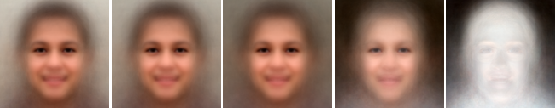
\includegraphics[width=\textwidth]{fig/PCA/pca1}
        \caption{Second Principal Component}
    \end{subfigure}
    \begin{subfigure}[b]{\textwidth}
        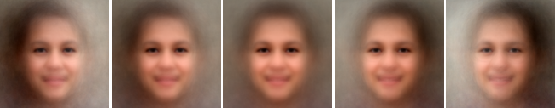
\includegraphics[width=\textwidth]{fig/PCA/pca2}
        \caption{Third Principal Component}
    \end{subfigure}
    \begin{subfigure}[b]{\textwidth}
        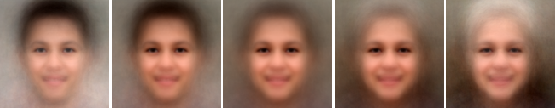
\includegraphics[width=\textwidth]{fig/PCA/pca3}
        \caption{Fourth Principal Component}
    \end{subfigure}
    \begin{subfigure}[b]{\textwidth}
        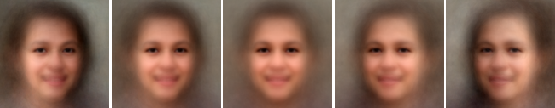
\includegraphics[width=\textwidth]{fig/PCA/pca4}
        \caption{Fifth Principal Component}
    \end{subfigure}
    \begin{subfigure}[b]{\textwidth}
        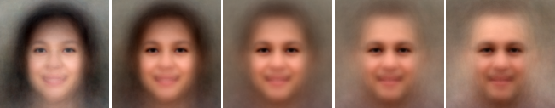
\includegraphics[width=\textwidth]{fig/PCA/pca5}
        \caption{Sixth Principal Component}
    \end{subfigure}
    \caption{Synthetic faces created by varying a single principal component to the mean face.}
    \label{pca-components}
\end{figure}

\section{DCGAN}


\begin{figure}
    \centering
    \begin{subfigure}[b]{0.45\textwidth}
        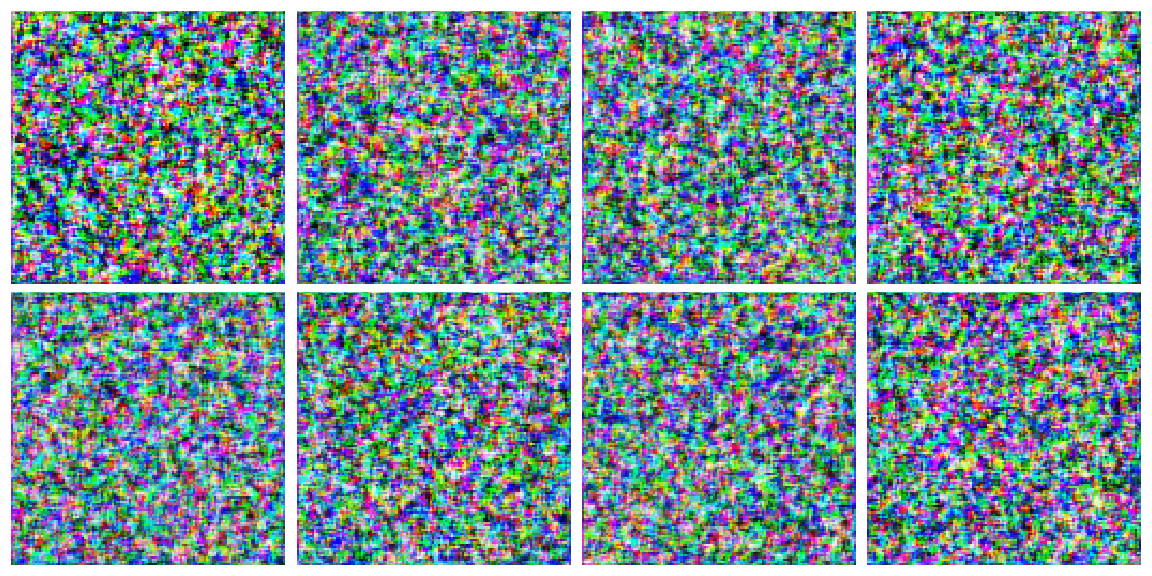
\includegraphics[width=\textwidth]{fig/dcgan/ffhq/epoch0}
        \caption{Epoch 0}
    \end{subfigure}
    ~
    \begin{subfigure}[b]{0.45\textwidth}
        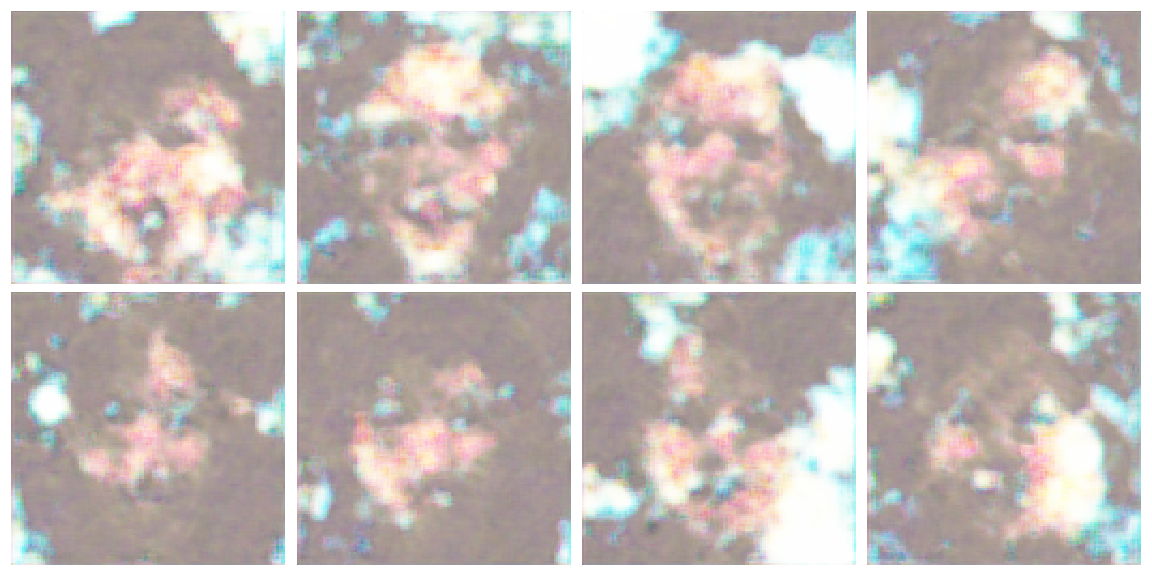
\includegraphics[width=\textwidth]{fig/dcgan/ffhq/epoch200}
        \caption{Epoch 10}
    \end{subfigure}

    \begin{subfigure}[b]{0.45\textwidth}
        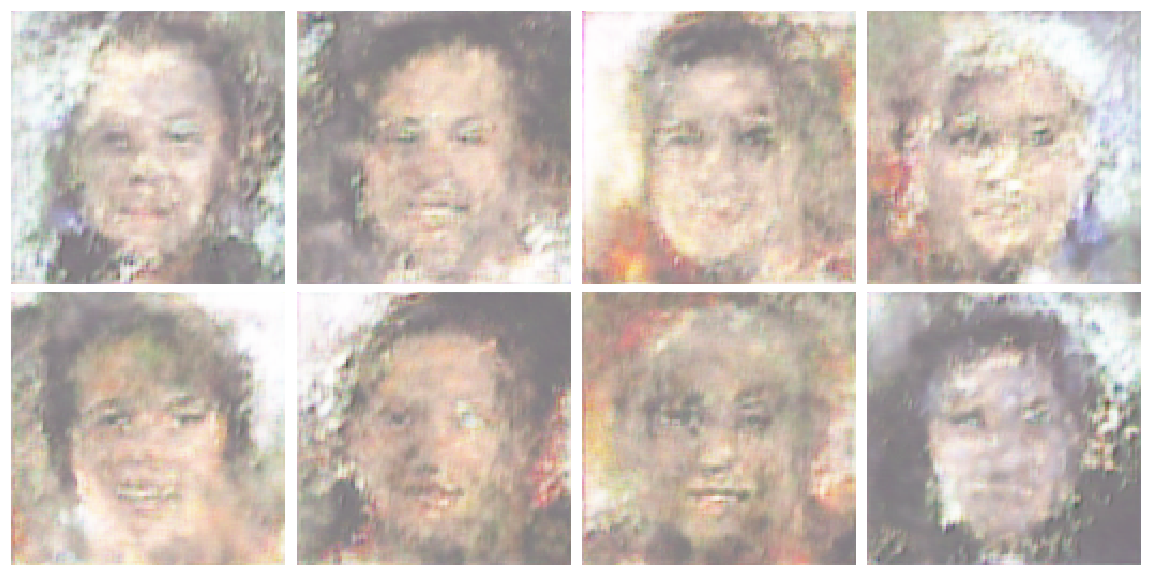
\includegraphics[width=\textwidth]{fig/dcgan/ffhq/epoch2000}
        \caption{Epoch 200}
    \end{subfigure}
    ~
    \begin{subfigure}[b]{0.45\textwidth}
        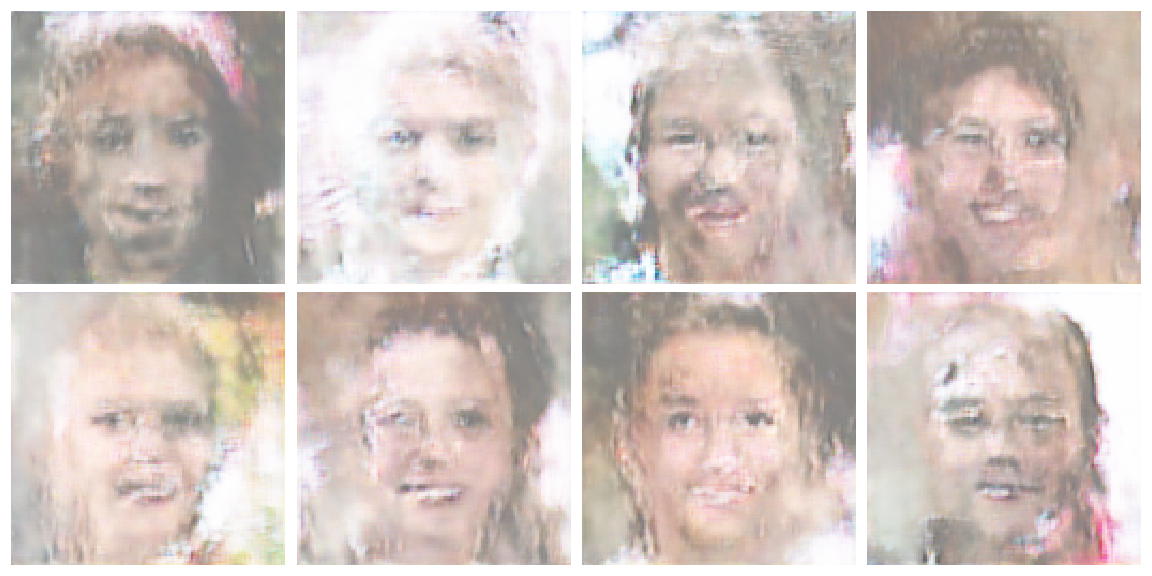
\includegraphics[width=\textwidth]{fig/dcgan/ffhq/epoch4000}
        \caption{Epoch 400}
    \end{subfigure}

    \begin{subfigure}[b]{\textwidth}
        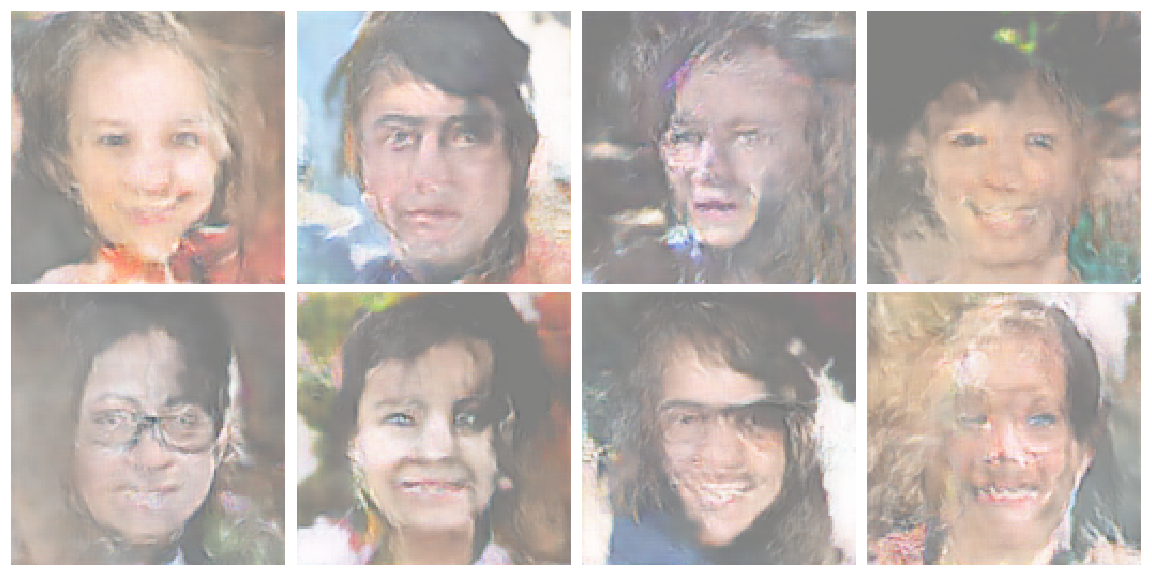
\includegraphics[width=\textwidth]{fig/dcgan/ffhq/epoch10000}
        \caption{Epoch 400}
    \end{subfigure}
    \caption{Samples from DCGAN during training on the FFHQ dataset}
    \label{dcgan-ffhq-samples}
\end{figure}

\begin{figure}

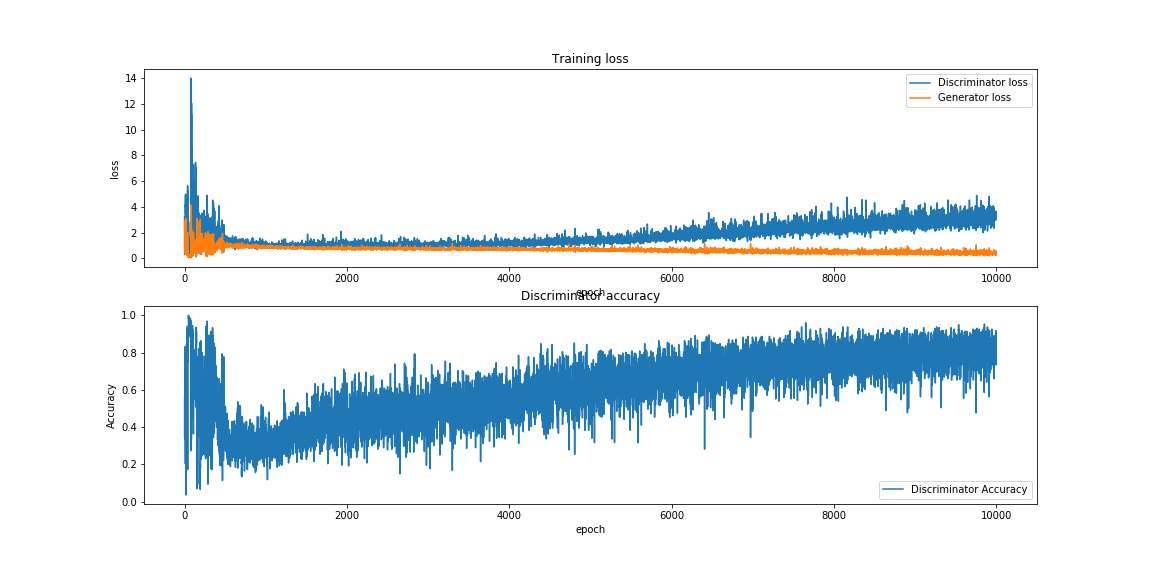
\includegraphics[width=\textwidth]{fig/dcgan/ffhq/loss}
  \caption{Loss and accuracy of the discriminator during training on the FFHQ Datase}
  \label{dcgan-ffhq-loss}
\end{figure}

\begin{figure}
    \centering
    \begin{subfigure}[b]{0.45\textwidth}
        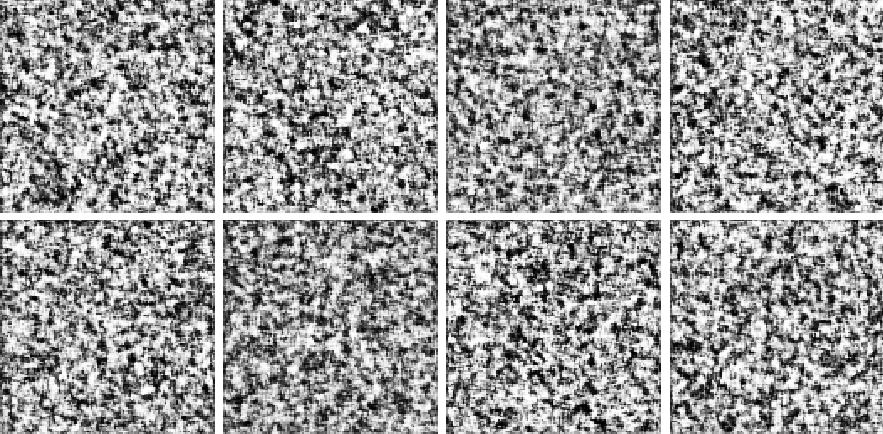
\includegraphics[width=\textwidth]{fig/dcgan/caltech/epoch0}
        \caption{Epoch 0}
    \end{subfigure}
    ~
    \begin{subfigure}[b]{0.45\textwidth}
        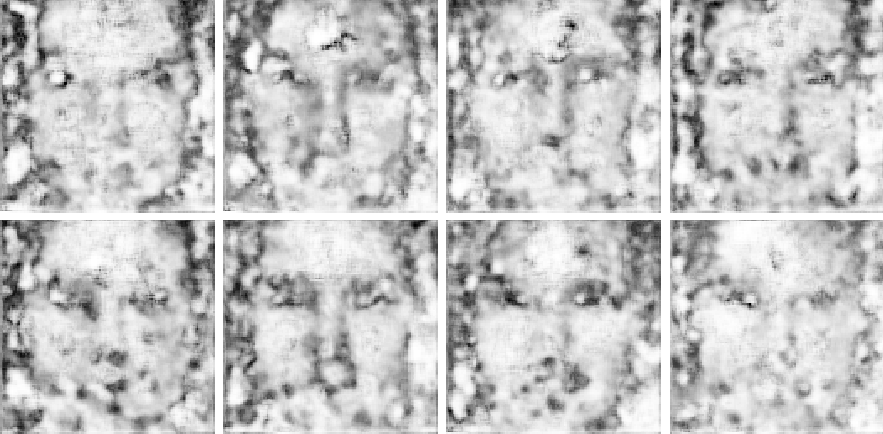
\includegraphics[width=\textwidth]{fig/dcgan/caltech/epoch200}
        \caption{Epoch 10}
    \end{subfigure}

    \begin{subfigure}[b]{0.45\textwidth}
        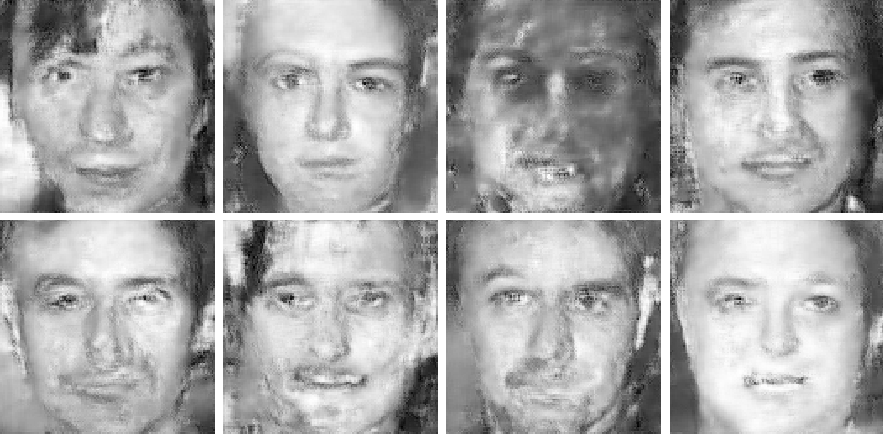
\includegraphics[width=\textwidth]{fig/dcgan/caltech/epoch2000}
        \caption{Epoch 200}
    \end{subfigure}
    ~
    \begin{subfigure}[b]{0.45\textwidth}
        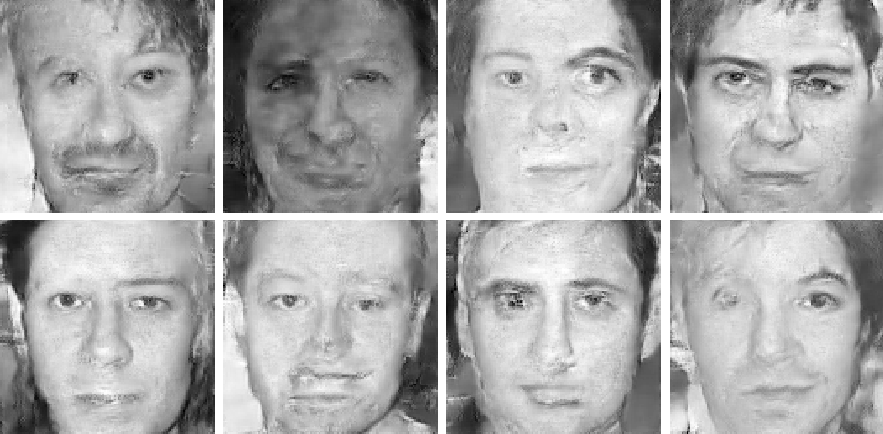
\includegraphics[width=\textwidth]{fig/dcgan/caltech/epoch4000}
        \caption{Epoch 400}
    \end{subfigure}

    \begin{subfigure}[b]{\textwidth}
        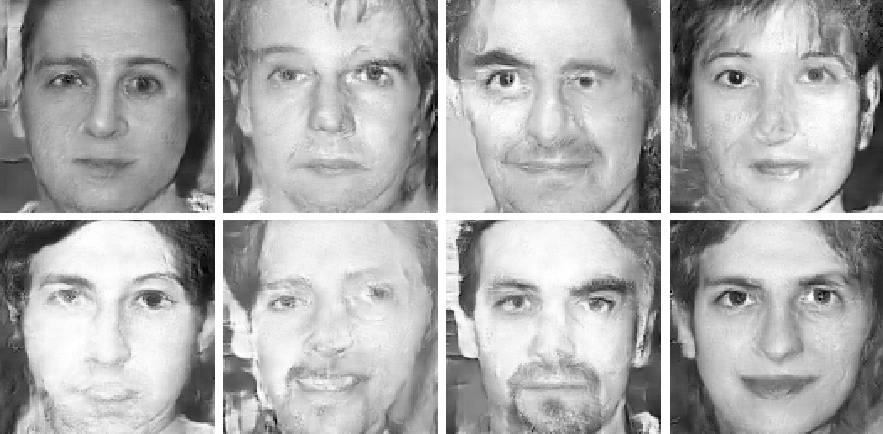
\includegraphics[width=\textwidth]{fig/dcgan/caltech/epoch10000}
        \caption{Epoch 400}
    \end{subfigure}
    \caption{Samples from DCGAN during training on the Caltech dataset}
    \label{dcgan-caltech-samples}
\end{figure}

\begin{figure}

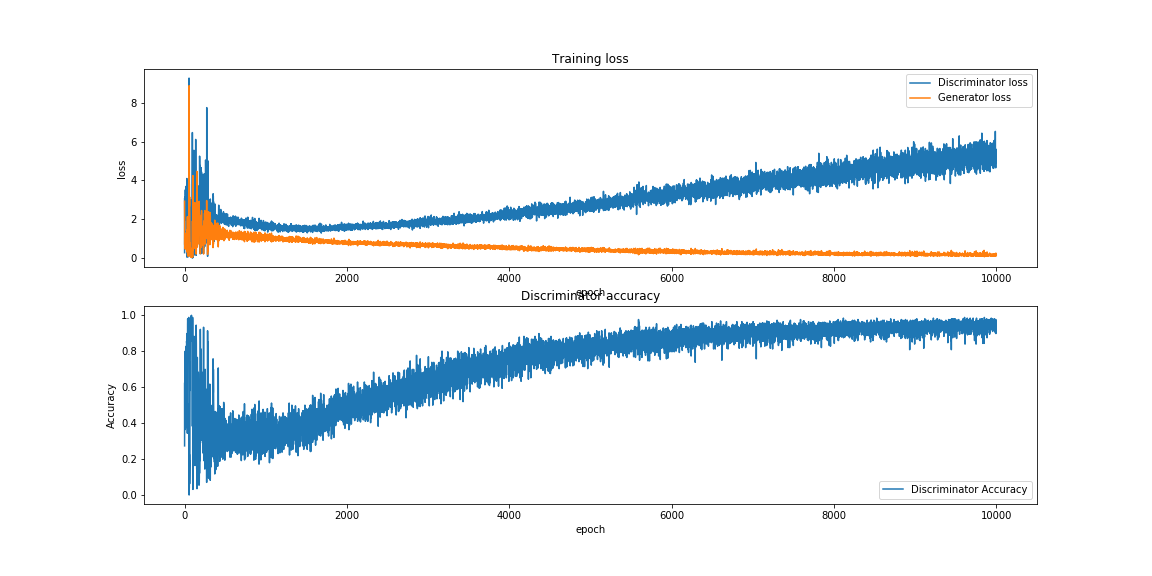
\includegraphics[width=\textwidth]{fig/dcgan/caltech/loss}
  \caption{Loss and accuracy of the discriminator during training on the Caltech Dataset}
  \label{dcgan-caltech-loss}
\end{figure}



% \begin{figure}
%     \centering
%     \begin{subfigure}[b]{0.3\textwidth}
%         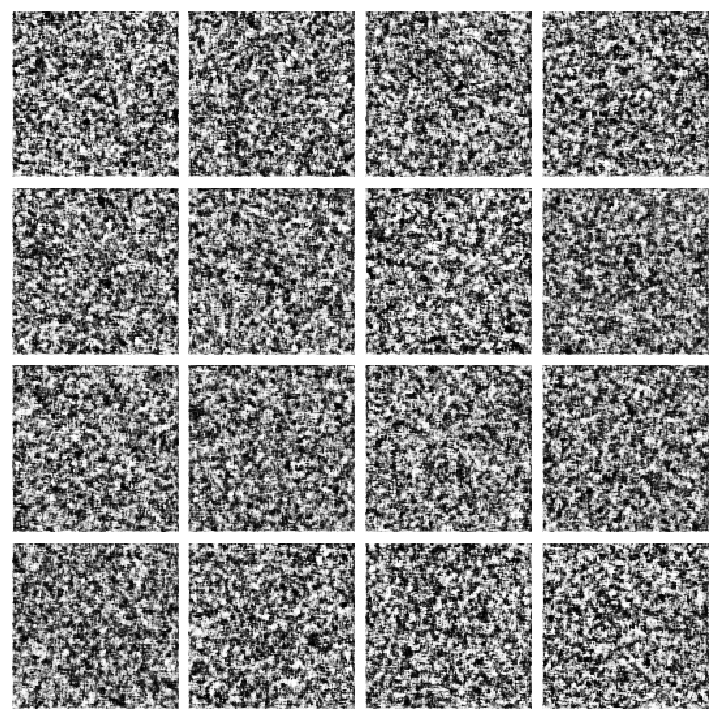
\includegraphics[width=\textwidth]{fig/dcgan/epoch0}
%         \caption{Epoch 0}
%     \end{subfigure}
%     ~
%     \begin{subfigure}[b]{0.3\textwidth}
%         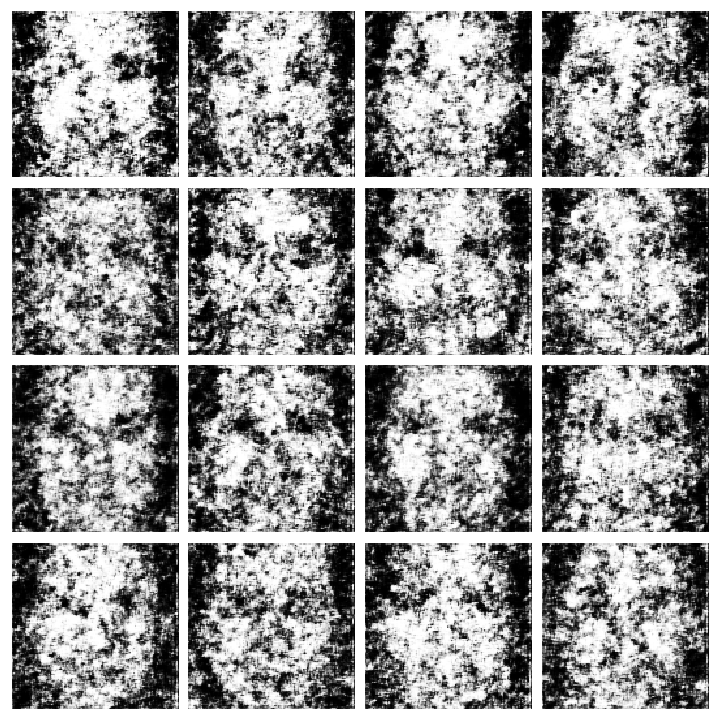
\includegraphics[width=\textwidth]{fig/dcgan/epoch10}
%         \caption{Epoch 10}
%     \end{subfigure}
%     ~
%     \begin{subfigure}[b]{0.3\textwidth}
%         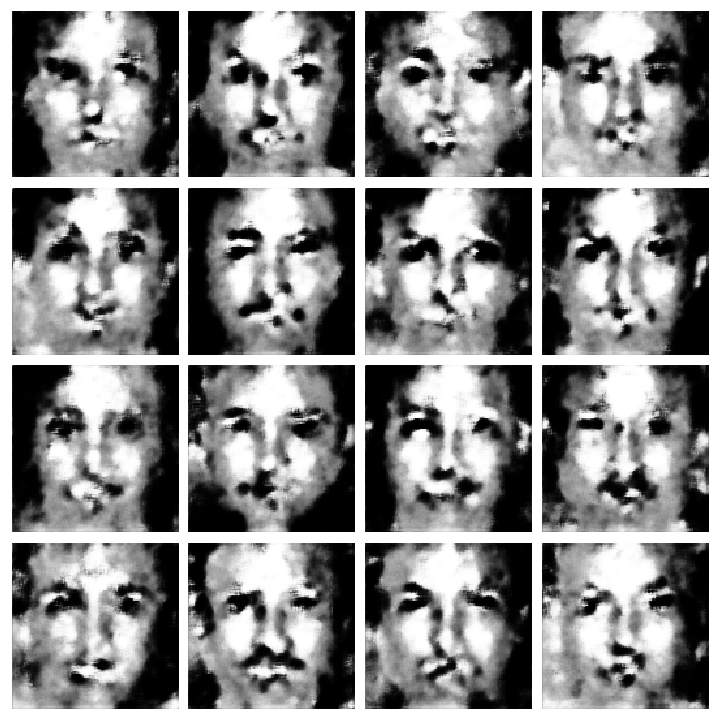
\includegraphics[width=\textwidth]{fig/dcgan/epoch100}
%         \caption{Epoch 100}
%     \end{subfigure}
%
%     \begin{subfigure}[b]{0.3\textwidth}
%         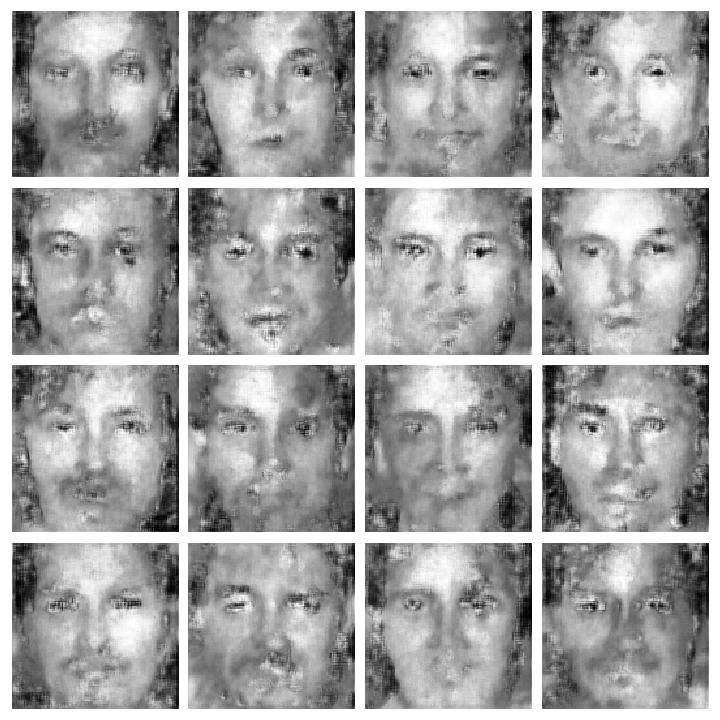
\includegraphics[width=\textwidth]{fig/dcgan/epoch200}
%         \caption{Epoch 200}
%     \end{subfigure}
%     ~
%     \begin{subfigure}[b]{0.3\textwidth}
%         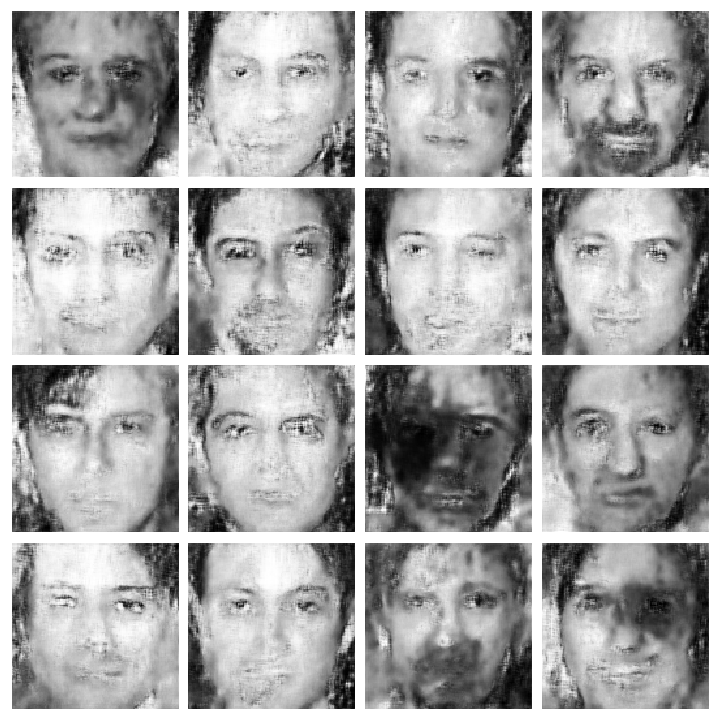
\includegraphics[width=\textwidth]{fig/dcgan/epoch400}
%         \caption{Epoch 400}
%     \end{subfigure}
%     ~
%     \begin{subfigure}[b]{0.3\textwidth}
%         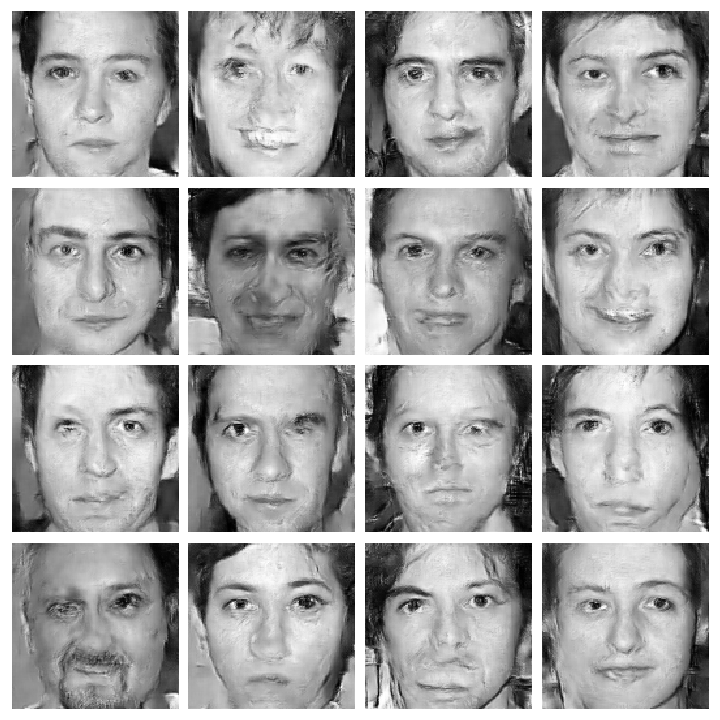
\includegraphics[width=\textwidth]{fig/dcgan/epoch4000}
%         \caption{Epoch 4000}
%     \end{subfigure}
%
%     \caption{Samples from DCGAN during traning on the Caltech dataset}
% \end{figure}

\section{StyleGAN}

We can download the weigths of a pre-trained stylegan trained by Nvidia\footnote{\url{
https://github.com/NVlabs/stylegan.git}}\cite{stylegan}

\begin{figure}
  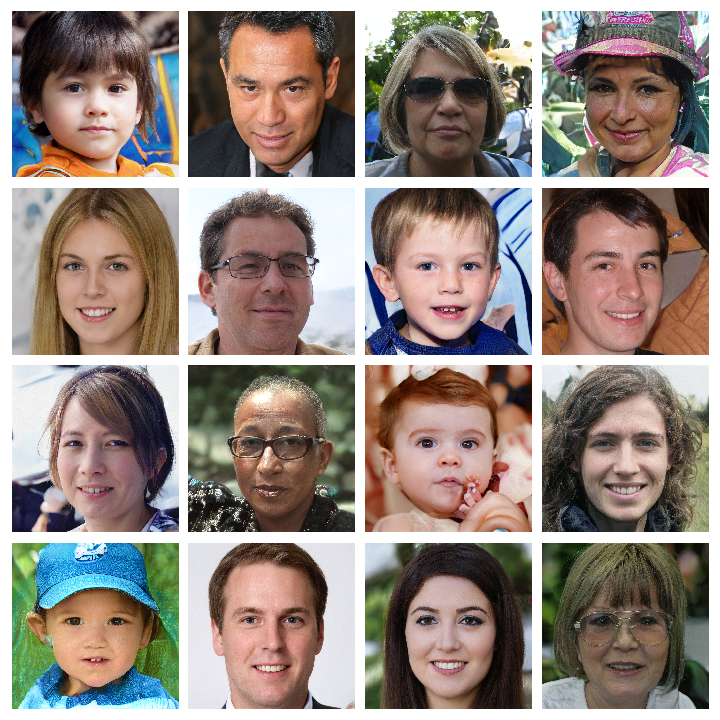
\includegraphics[width=\textwidth]{fig/stylegan/stylegan_example}
  \caption{Random samples from the pretrained StyleGAN}
  \label{StyleGAN-examples}
\end{figure}


\begin{figure}
  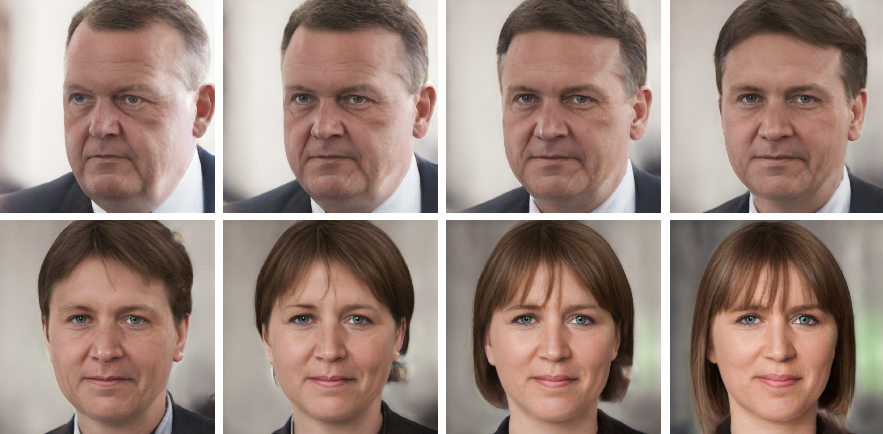
\includegraphics[width=\textwidth]{fig/stylegan/interpolation}
  \caption{Interpolation between two StyleGAN images}
  \label{StyleGAN-interpolation}
\end{figure}


\subsection{Finding the latent space representation of an arbitrary query image.}
Now the pretrained StyleGAN does not contain any encoder network. Therefore there is no way to find a latent space representation of a arbitrary input image.
There is, however a a least two different ways of tackling this problem.
%
% One is the optimization-based
% approach, which directly optimizes the latent code with fixed generator to minimize the pixel-wise reconstruction error [22]. The other is the encoder-based, where an independent encoder network is trained to learn the inverse mapping [37].
\cite{interfacegan}
The paper \textit{Image2StyleGAN: How to Embed Images Into the StyleGAN Latent Space?}\cite{Image2StyleGAN} explicitly investigates this problem.


Here we use the first approach where hold the pretrained generator fixed and then optimize the latent vector to give the desired output image. But instead of calculating the loss directly on the pixel-wise recontruction error.
\footnote{https://github.com/Puzer/stylegan-encoder}



Here we use the same approach as in \cite{styletransfer} where



We use a pre-trained VGG16 network for transforming a query image and the generated image from the latent vector into a high dimensional feature space. The loss is them calculated as a difference between the two feature vectors in the VGG16 feature space.

% Optimization is performed only for latent representation which we want to obtain.

% Upon completion of optimization you are able to transform your latent vector as you wish. For example you can find a "smiling direction" in your latent space, move your latent vector in this direction and transform it back to image using the generator.

%
% \begin{figure}[htb]
%     \centering
%     \begin{subfigure}[b]{\textwidth}
%         \centering
%         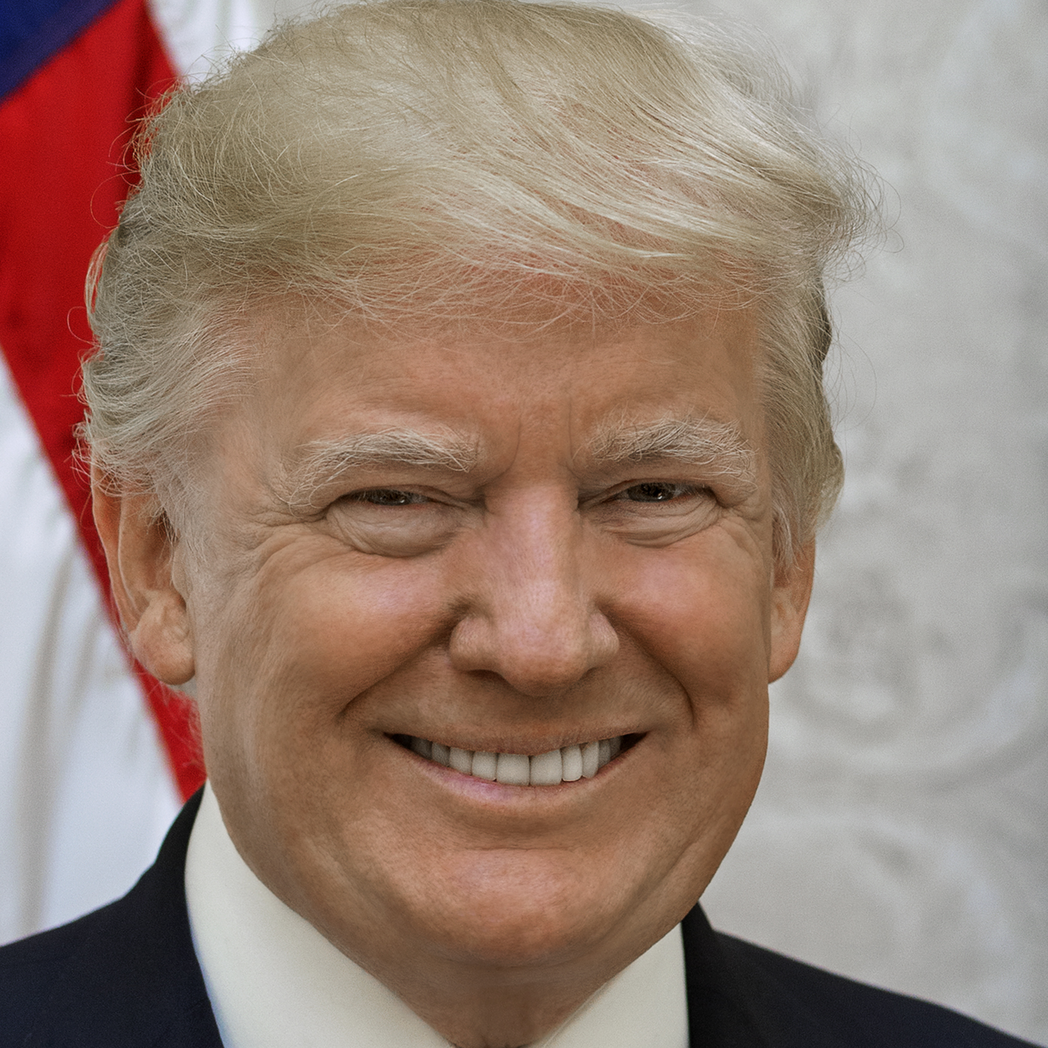
\includegraphics[width=0.3\linewidth]{fig/query_images/trump}%
%         \hfill
%         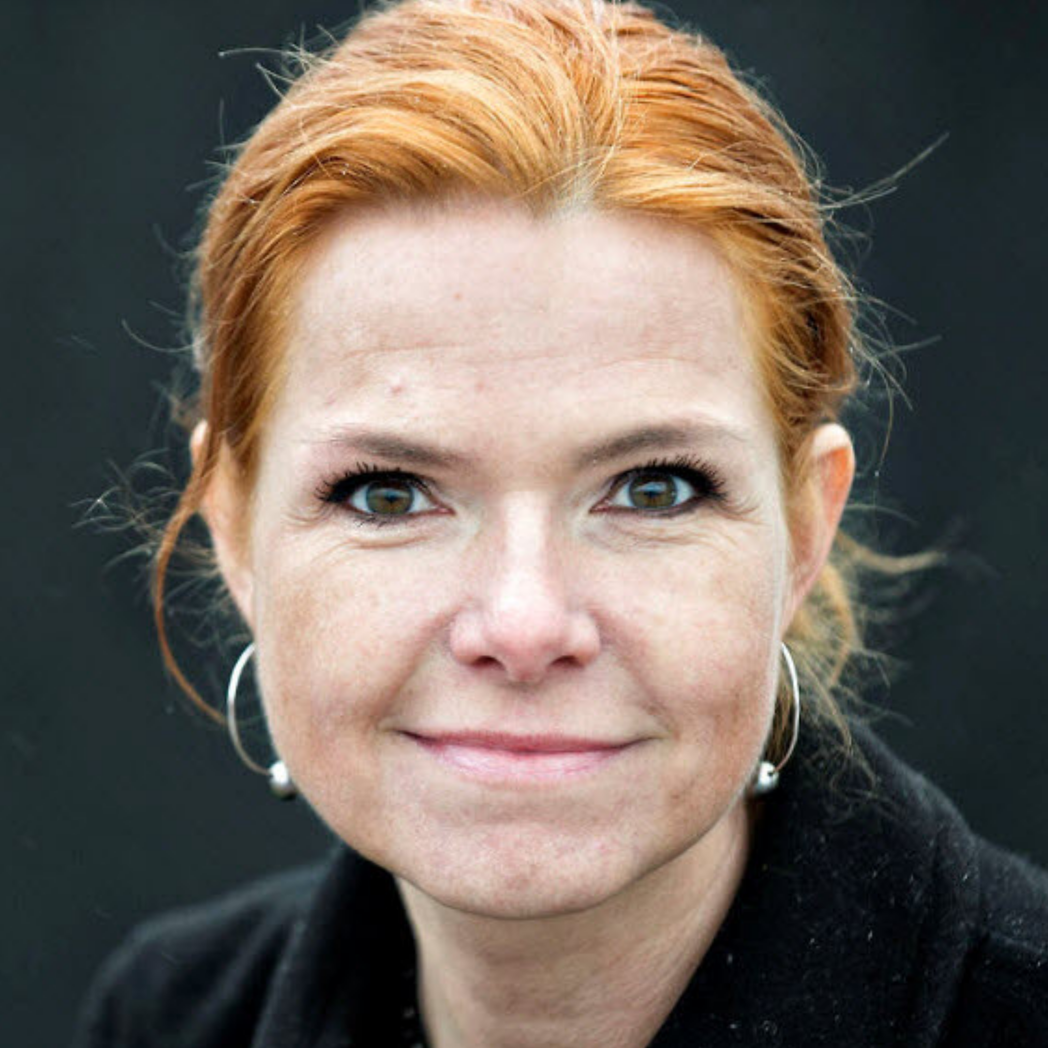
\includegraphics[width=0.3\linewidth]{fig/query_images/inger}
%         \hfill
%         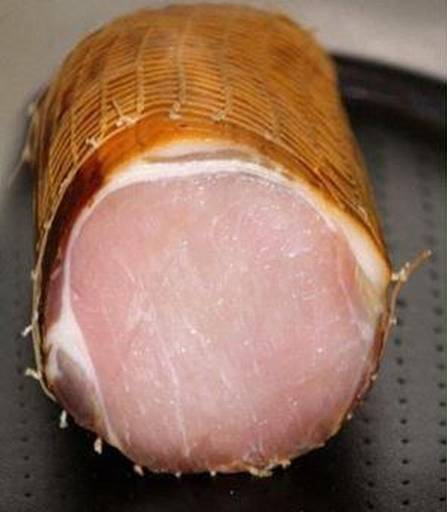
\includegraphics[width=0.3\linewidth]{fig/query_images/skinke}
%         \caption{Original Query Images}
%     \end{subfigure}
%     \vskip\baselineskip
%     \begin{subfigure}[b]{\textwidth}
%         \centering
%         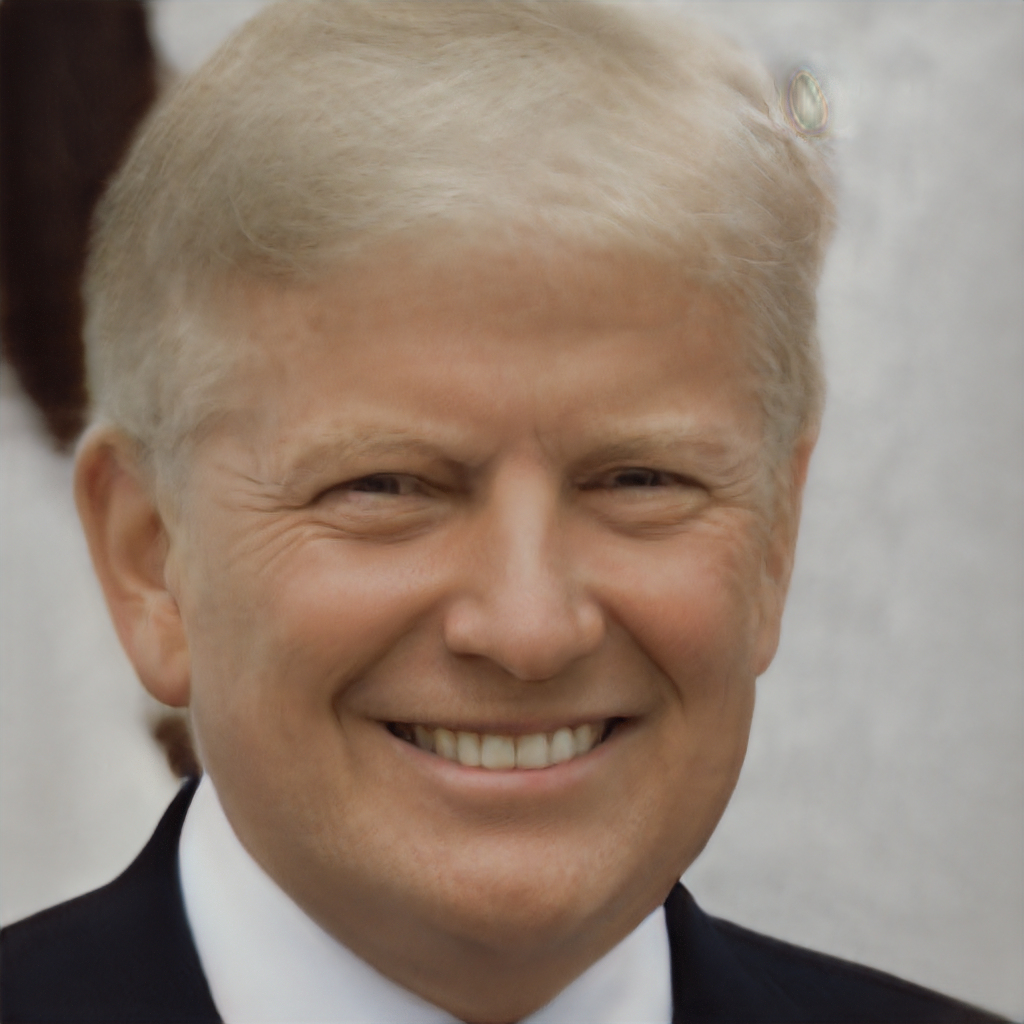
\includegraphics[width=0.3\linewidth]{fig/query_images_reconstucted/trump}%
%         \hfill
%         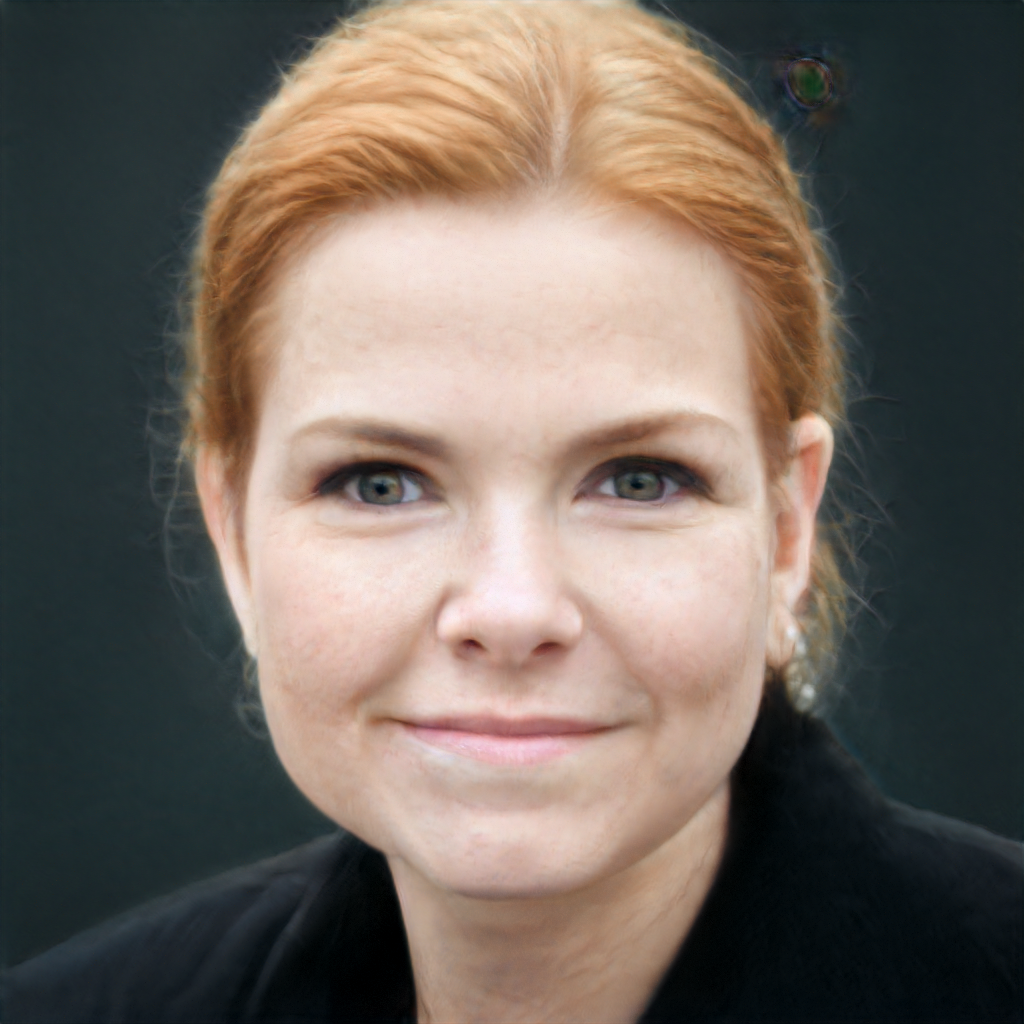
\includegraphics[width=0.3\linewidth]{fig/query_images_reconstucted/inger}
%         \hfill
%         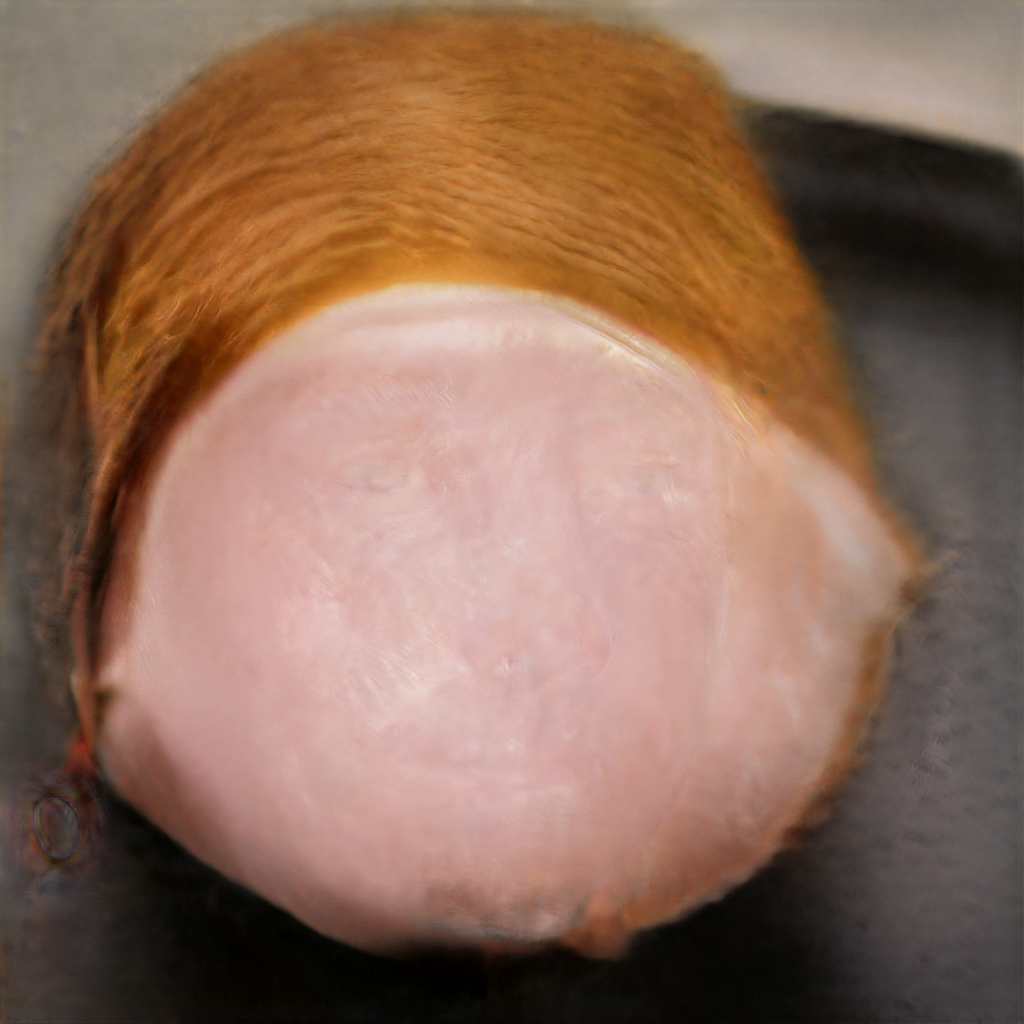
\includegraphics[width=0.3\linewidth]{fig/query_images_reconstucted/skinke}
%         \caption{Reconstructed images from StyleGAN latent space}
%     \end{subfigure}
%     \caption{Latent space representation of arbitrary query images }
% \end{figure}

% \begin{figure}
%     \centering
%     \begin{subfigure}[b]{0.45\textwidth}
%         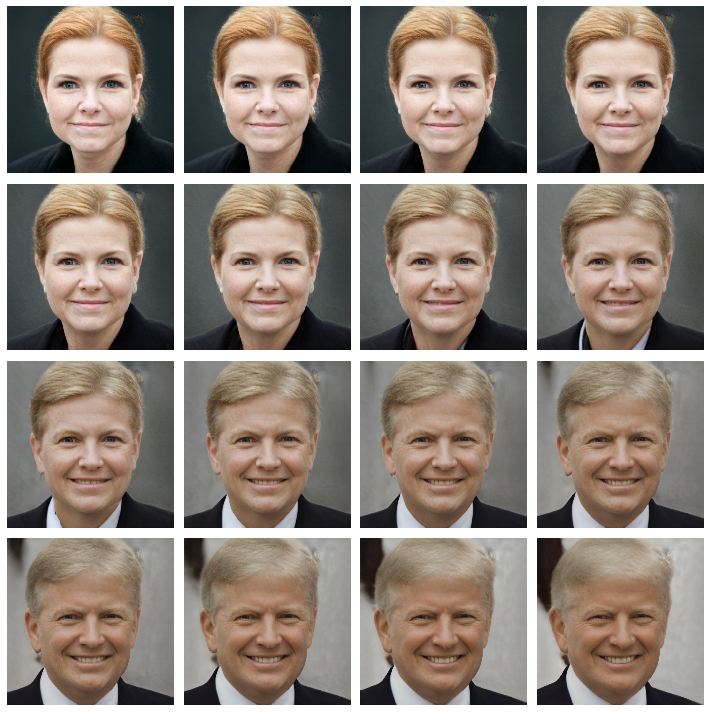
\includegraphics[width=\textwidth]{fig/ingertrump}
%         \caption{Inger Støjberg to Donald Trump}
%     \end{subfigure}
%     ~
%     \begin{subfigure}[b]{0.45\textwidth}
%         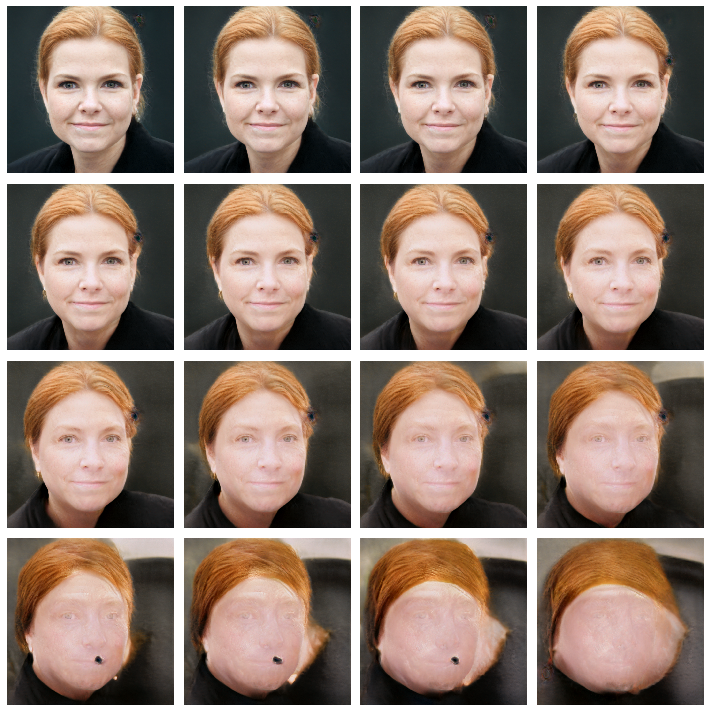
\includegraphics[width=\textwidth]{fig/ingerham}
%         \caption{Inger Støjberg to Ham}
%     \end{subfigure}
%     \caption{Interpolations between query images in the StyleGAN latent space.}
% \end{figure}


\subsection{Semantic face editing.}
